\section{Demographics Driven Map Distortion Method}

\subsection{Data-driven Profile Design}

Figure~\ref{fig:design_profile} shows the legend for the user profile. Those design dimensions are driven by data. an intuitive perception of the social characteristics. 

\begin{figure}[htb!]
 \centering % avoid the use of \begin{center}...\end{center} and use \centering instead (more compact)
 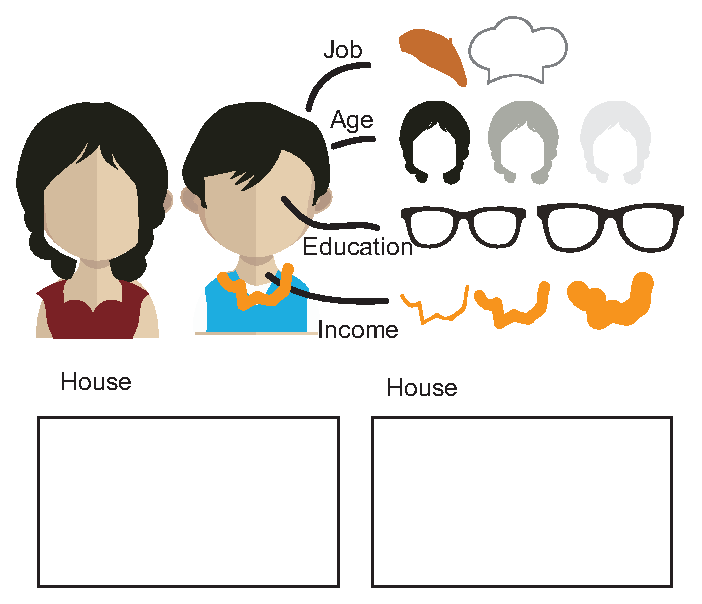
\includegraphics[width=\columnwidth]{pictures/design_profile}
 \caption{Design Profile}
 \label{fig:design_profile}
\end{figure}

Various profiles are generated. Figure~\ref{fig:div_profile} shows some results.


\begin{figure}[htb!]
 \centering % avoid the use of \begin{center}...\end{center} and use \centering instead (more compact)
 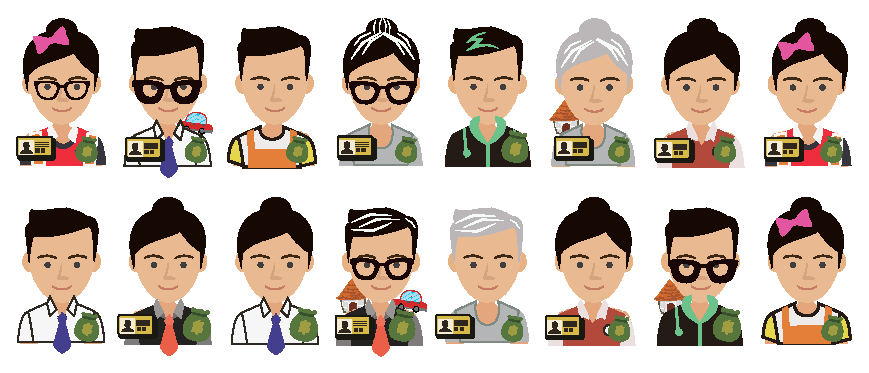
\includegraphics[width=\columnwidth]{pictures/design_div}
 \caption{Diverse Profile}
 \label{fig:div_profile}
\end{figure}

\subsection{Interactive Group Classification}

Figure~\ref{fig:mds} is the MDS project of diversse users. Contour detected. Classification Updated. Automatic ensembling of diverse profiles. 


\begin{figure}[htb!]
 \centering % avoid the use of \begin{center}...\end{center} and use \centering instead (more compact)
 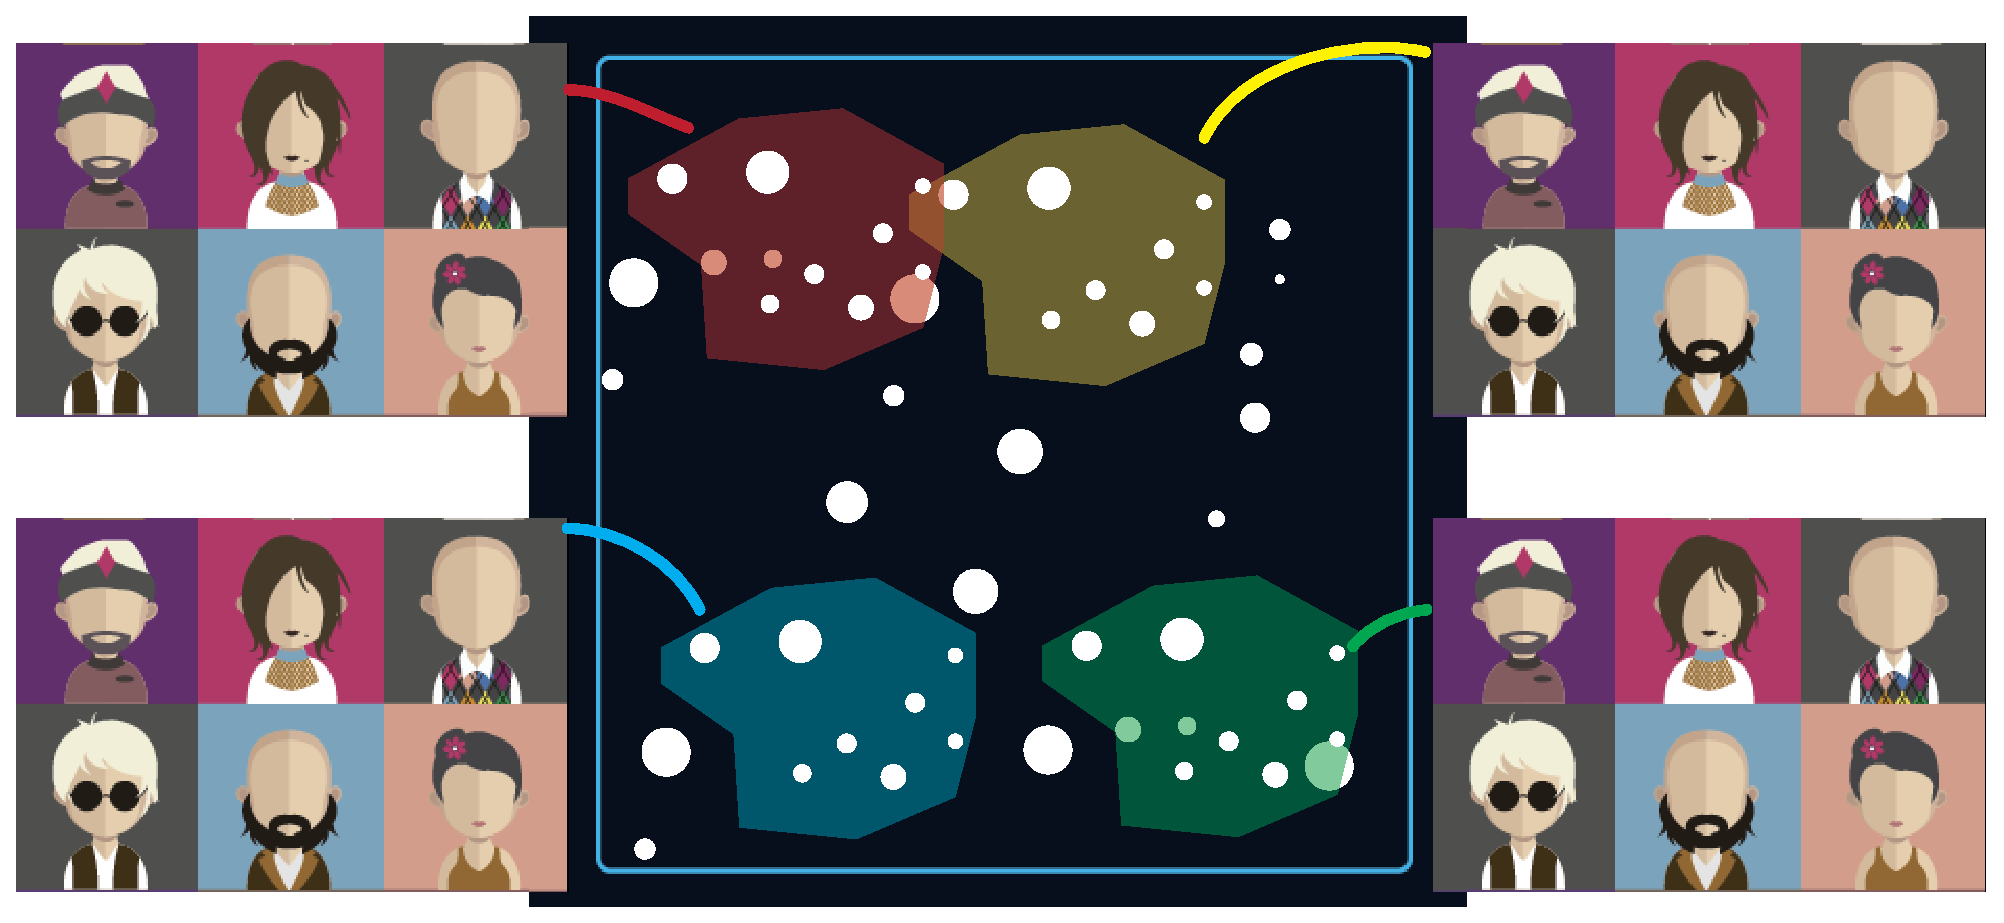
\includegraphics[width=\columnwidth]{pictures/mds}
 \caption{Interactive Labelling and Classification}
 \label{fig:mds}
\end{figure}